\documentclass[10pt]{article}
\usepackage[T1]{fontenc}
\usepackage[margin=0.72in]{geometry}
\usepackage{amsmath,amssymb,amsthm}
\usepackage{graphicx}
\usepackage[colorlinks=true,linkcolor=blue,citecolor=blue,urlcolor=blue]{hyperref}
\usepackage{microtype}

\newtheorem{theorem}{Theorem}
\newtheorem{lemma}{Lemma}
\newcommand{\R}{\mathbb R}
\newcommand{\Om}{\Omega_1^+}
\newcommand{\supp}{\operatorname{supp}}

\title{Triangle--Gaussian convolution preserves\\
extremality}
\author{Full answer to the first clause of Question 3 in arXiv:0801.0941\\
Routed from the open problem in arXiv:1803.06409}
\date{13 August 2026}

\begin{document}
\maketitle

\noindent\textbf{Status.}
The first clause of Question 3 has an affirmative answer:
\[
 f(x)=(1-|x|)_+,\qquad \gamma(x)=e^{-\pi x^2}
 \quad\Longrightarrow\quad f*\gamma\text{ is extremal in }\Om.
\]
Together with this run's existing counterexample to the second clause, this
completes the explicit two-part question.

\section*{Source route and exact question}

The queue source states that describing the extreme rays of the cone of
nonnegative positive-definite \(C_0(\R)\) functions is open and directs the
reader to Jaming--Matolcsi--R\'ev\'esz \cite[p.~9]{GKR}.

\begin{center}
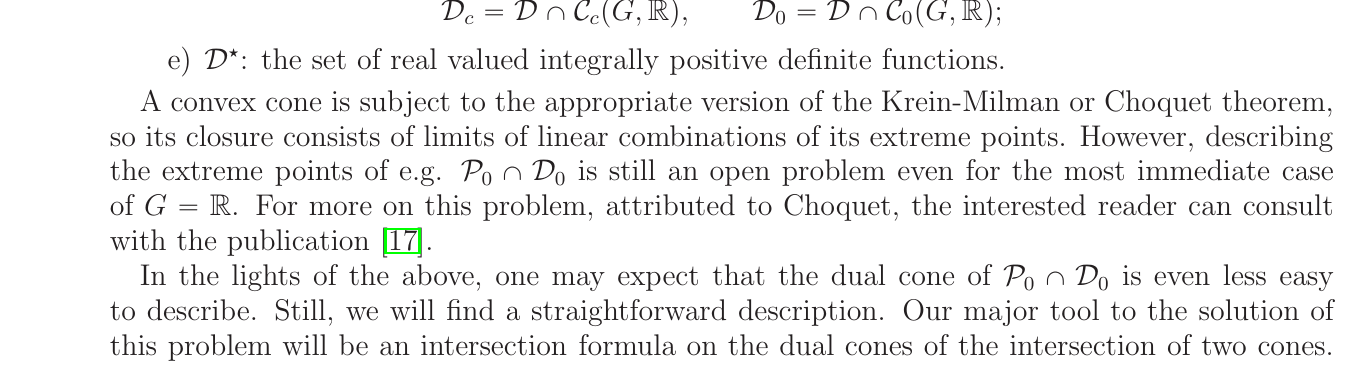
\includegraphics[width=0.94\textwidth]{source/route_open_problem_page9.png}
\end{center}
\vspace{-0.8em}
\noindent\emph{Routing evidence: arXiv:1803.06409, PDF page 9.}

The cited paper defines \(\Om\) as the cone of continuous nonnegative
positive-definite functions on \(\R\).  It recalls that the triangle
\[
 f=\mathbf1_{[-1/2,1/2]}*\mathbf1_{[-1/2,1/2]}=(1-|x|)_+
\]
and \(\gamma=e^{-\pi x^2}\) are extremal, and asks first whether
\(f*\gamma\) is extremal \cite[p.~18, Question 3]{JMR}.

\begin{center}
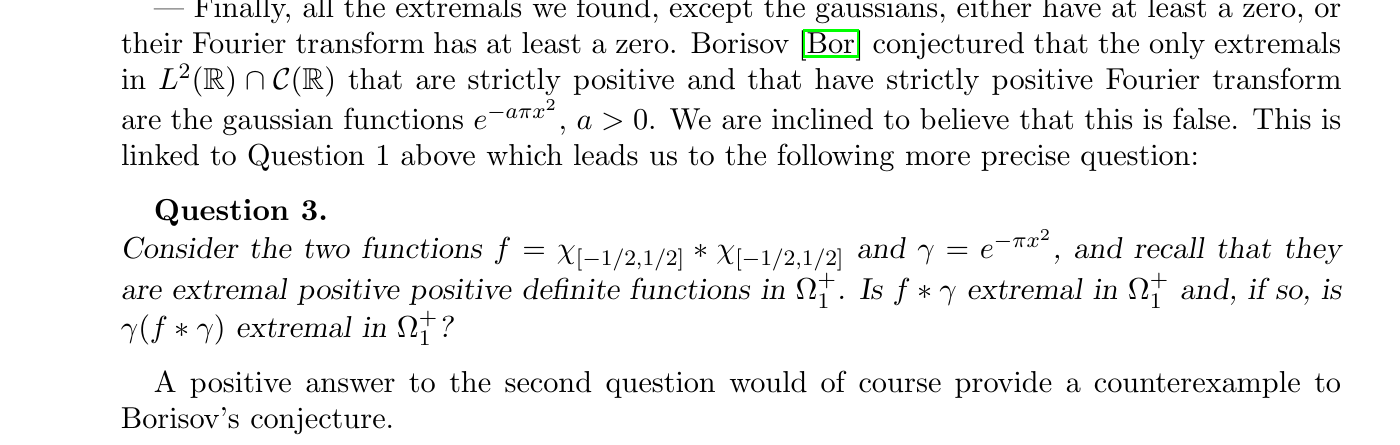
\includegraphics[width=0.94\textwidth]{source/question3_page18.png}
\end{center}
\vspace{-0.7em}
\noindent\emph{Exact source question: arXiv:0801.0941, PDF page 18.}

We use
\[
 \widehat a(\xi)=\int_\R a(x)e^{-2\pi i x\xi}\,dx,
 \qquad
 F(\xi):=\widehat f(\xi)=
 \left(\frac{\sin\pi\xi}{\pi\xi}\right)^2,
 \qquad \widehat\gamma=\gamma.
\]

\section*{Answer}

\begin{theorem}\label{thm:main}
The function \(h=f*\gamma\) generates an extremal ray of \(\Om\).  That is,
if \(g,h-g\in\Om\), then \(g=\lambda h\) for some \(0\le\lambda\le1\).
\end{theorem}

\paragraph{Proof intuition.}
An interval component \(0\le g\le f*\gamma\) also satisfies the Fourier-side
inequality \(0\le\widehat g\le F\gamma\).  Removing the nowhere-zero Gaussian
factor defines a bounded ``initial datum'' \(u\) with \(g=u*\gamma\).  A
critical Phragm\'en--Lindel\"of/Paley--Wiener lemma says that domination by
the heat evolution of a function supported on \([-1,1]\) forces \(u\) to
have the same support bound.  Thus \(\widehat u\) is entire of the same
exponential type as \(F\).  Its nonnegativity makes it vanish to even order
at every nonzero integer, exactly where the sinc square has double zeros.
The quotient by \(F\) is therefore entire, has polynomial growth, and is
bounded on the real axis; it must be constant.

\section*{A Gaussian domination support lemma}

\begin{lemma}\label{lem:support}
Let \(u\) be bounded on \(\R\), let \(a\ge0\) be integrable with
\(\supp a\subseteq[-R,R]\), and suppose
\begin{equation}\label{eq:domination}
          0\le (u*\gamma)(x)\le(a*\gamma)(x)\qquad(x\in\R).
\end{equation}
Then \(\supp u\subseteq[-R,R]\).
\end{lemma}

\begin{proof}
Put \(v(t)=u(t)e^{-\pi t^2}\in L^1\cap L^2\), and define
\[
 L(z)=\int_\R v(t)e^{2\pi zt}\,dt\qquad(z\in\mathbb C).
\]
This is entire and the Gaussian integral gives
\begin{equation}\label{eq:crude}
             |L(x+iy)|\le C e^{\pi x^2}.
\end{equation}
Completing the square in \eqref{eq:domination} gives, for real \(x\),
\begin{align}
 0\le L(x)
 &=e^{\pi x^2}(u*\gamma)(x)\notag\\
 &\le\int_{-R}^{R}a(t)e^{-\pi t^2}e^{2\pi xt}\,dt
 \le C e^{2\pi R|x|}.                                      \label{eq:realbound}
\end{align}
Also \(|L(iy)|\le\|v\|_1\).

For completeness, we record the critical-order step that converts these
axial bounds into a Paley--Wiener bound.  Let
\[
 \mathfrak h(\theta)=\limsup_{r\to\infty}
 r^{-2}\log|L(re^{i\theta})|
\]
be the order-two indicator.  Equation \eqref{eq:crude} gives
\(\mathfrak h(\theta)\le\pi\cos^2\theta\), while the improved bounds give
\(\mathfrak h(0),\mathfrak h(\pi/2)\le0\).  Fix
\(0<\theta<\pi/2\) and put \(\beta=\pi/2-\delta>\theta\).  The standard
two-trigonometric convexity of the indicator on a sector of width less than
\(\pi/2\) yields
\[
 \mathfrak h(\theta)
 \le\frac{\mathfrak h(0)\sin2(\beta-\theta)
          +\mathfrak h(\beta)\sin2\theta}{\sin2\beta}
 \le\frac{\pi\sin^2\delta}{\sin2\delta}\sin2\theta.
\]
Letting \(\delta\downarrow0\) proves \(\mathfrak h\le0\) in that quadrant;
the other three are identical.  Thus \(L\) is of order at most two and
minimal type.  The critical Phragm\'en--Lindel\"of theorem, applied in the
right quadrants to \(L(z)e^{-2\pi Rz}\) and in the left quadrants to
\(L(z)e^{2\pi Rz}\), now gives
\begin{equation}\label{eq:type}
                     |L(z)|\le C e^{2\pi R|\Re z|}.
\end{equation}
Indeed, each modified function has minimal type and is bounded on both rays
forming the relevant quadrant by \eqref{eq:realbound} and the imaginary-axis
bound.

The entire function \(W(\zeta)=L(-i\zeta)\) is therefore of exponential
type at most \(2\pi R\), and \(W|_\R\) is the Fourier transform of the
\(L^2\)-function \(v\).  The \(L^2\) Paley--Wiener theorem gives
\(\supp v\subseteq[-R,R]\).  Since \(e^{-\pi t^2}\) never vanishes,
\(\supp u=\supp v\), proving the lemma.
\end{proof}

\section*{Proof of Theorem~\ref{thm:main}}

Suppose \(g,h-g\in\Om\).  Then \(0\le g\le h\), so both summands are
integrable.  Their positive definiteness gives
\begin{equation}\label{eq:fourierinterval}
 0\le G(\xi):=\widehat g(\xi)
 \le\widehat h(\xi)=F(\xi)e^{-\pi\xi^2}\qquad(\xi\in\R).
\end{equation}
Define
\[
                         U(\xi)=e^{\pi\xi^2}G(\xi).
\]
By \eqref{eq:fourierinterval}, \(0\le U\le F\).  Since \(F\in L^1\),
also \(U\in L^1\).  Let \(u=\check U\); then \(u\) is bounded and
continuous, and Fourier inversion gives
\[
                             g=u*\gamma.
\]
Lemma~\ref{lem:support}, applied with \(a=f\) and \(R=1\), gives
\(\supp u\subseteq[-1,1]\).  Thus
\[
 U(z)=\int_{-1}^{1}u(t)e^{-2\pi itz}\,dt
\]
extends to an entire function of exponential type at most \(2\pi\).

For every nonzero integer \(n\), \(F(n)=0\), so \(0\le U\le F\) gives
\(U(n)=0\).  Because \(U\) is real analytic and nonnegative on \(\R\), each
such zero has even order, hence order at least two.  The zeros of
\[
                         F(z)=\left(\frac{\sin\pi z}{\pi z}\right)^2
\]
are exactly those nonzero integers, all double.  Consequently
\[
                              Q(z)=\frac{U(z)}{F(z)}
\]
is entire.

Fix small disjoint disks about the nonzero integers.  Outside those disks,
the elementary lower bound for the sine gives
\[
 |F(z)|\ge c\frac{e^{2\pi|\Im z|}}{(1+|z|)^2},
 \qquad
 |U(z)|\le\|u\|_1e^{2\pi|\Im z|}.
\]
Hence \(|Q(z)|\le C(1+|z|)^2\) there.  The maximum principle on each
omitted disk supplies the same global bound.  Therefore \(Q\) is a
polynomial of degree at most two.  On \(\R\), however,
\[
                           0\le Q(x)=\frac{U(x)}{F(x)}\le1
\]
away from the zeros, and continuity fills in those points.  A polynomial
bounded on \(\R\) is constant.  Write \(Q\equiv\lambda\), where
\(0\le\lambda\le1\).  Then \(U=\lambda F\), so
\(G=\lambda Fe^{-\pi\xi^2}=\lambda\widehat h\).  Fourier injectivity gives
\(g=\lambda h\), proving extremality. \(\square\)

\section*{Scope and provenance}

This is a full affirmative answer to the first clause of Question 3, not a
classification of all extreme rays.  A separate existing packet in this run
proves the second clause false by an explicit perturbative decomposition.
Thus the two packets together answer both clauses: \(f*\gamma\) is extremal,
but \(\gamma(f*\gamma)\) is not.  Exact arXiv-id, title, quotation, formula,
product/convolution, and Borisov-conjecture searches through 13 August 2026
found no later answer to the first clause.  The proof above is a new result
of this run.

\begin{thebibliography}{9}
\bibitem{GKR}
M.~Ga\'al, S.~Nagy, and Sz.~Gy. R\'ev\'esz,
\emph{Integral comparisons of nonnegative positive definite functions on
LCA groups}, arXiv:1803.06409 (2018; revised 2019).

\bibitem{JMR}
P.~Jaming, M.~Matolcsi, and Sz.~Gy. R\'ev\'esz,
\emph{On the extremal rays of the cone of positive, positive definite
functions}, arXiv:0801.0941; J. Fourier Anal. Appl. 15 (2009), 561--582.
\end{thebibliography}

\end{document}
